\section{Sving}
For at bilen kan opdage og  gemme at der er et sving på banen, skal den udstyres med en sensor der kan kende forskel på ligeud kørsel og sving. Det vides at bilen bliver påvirket af en centripetalkraft, når den køre inde i et sving. For at kunne måle denne kraft, bruges der et accelerometer. Der var to accelerometer til rådighed, et digitalt (lis35de) og et analogt (mma1270keg). Først blev valget det digitale, da dette har en højere opløsning end det analoge. Grundet problemer med kommunikation mellem det digitale accelerometer, blev det fravalgt og det analoge accelerometer blev brugt i stedet.

\begin{figure}
\center
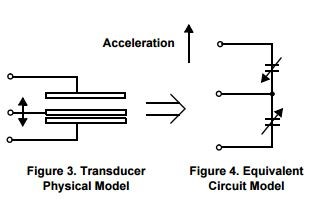
\includegraphics[scale=0.4]{./Graphics/Acceleration}
\caption{Accelerometer opbygning}
\label{Acceleration}
\end{figure}

\subsection{Hardware-mma1270keg}
Det analoge accelerometer er opbygget som vist på figur ?? $/todo{fil mma1270keg_Funk}$ . Det kan ses som tre plade hvor de to yderste er fikseret og den midterste kan bevæge sig.  Den midterste plade bevæger sig derved med kraften og capaciteten ændres mellem den midterste og de to fikserede plade. Dog er den samlede capacitans konstant. Dette kan beskrives ved $(C=\frac{A_{\epsilon}})$, hvor A er arealet af pladerne, $\epsilon$ er den diaelektriske konstant og D er afstanden mellem den midterste plade og en af de to fikserede plade. Denne capacitet bliver behandlet inde i accelerometeret, af et kredsløb ( Se side 4 i datablad for mma1270keg) Dette kredsløb sørger for at output signalet på accelerometetr er proportionalt med kraften.

\begin{wrapfigure}{r}{0.5\textwidth}
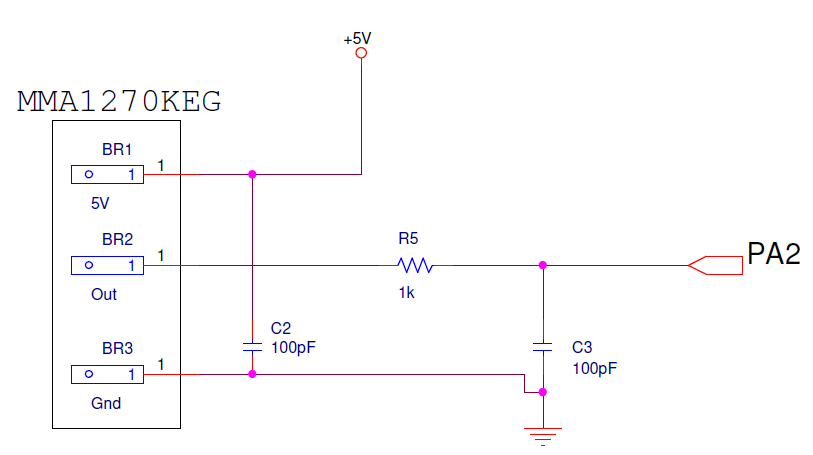
\includegraphics[scale=0.8]{./Graphics/Accelerometer_diagram}
\caption{Kredsløbs diagram over accelerometer}
\label{diagram_acc}
\end{wrapfigure}

Ved at se på Tabel 2 på side 3 i databladet for accelerometert, ses det at ved 0-G er outputtet typisk på 2.5  og en sensitivitet på $750\frac{mv}{g}$. /todo{Lav en graf for dette}
Output signalet, er et signal der ligge mellem 0-5v og kan læses med en ADC af microcontroleren.
Der er lavet er Lowpass filter på output signalet fra accelerometeret, for at sortere de høje frekvenser fra. Der blev konstrueret det samme som blev opfordret i databladet for sensoren. Altså en modstand på 1Kohm og en capacitor på 100 nF. Dette giver en cout-off frekvens på.\\$f_{c}=\frac{1}{2\pi\tau}=\frac{1}{2\pi*RC}=1591.5 HZ$\\

Dette Lowpass filter blev dog ikke optimeret grundet tidsmangel og der tages derfor højde for dette i koden.\\

\subsection{Software}
Til at læse sensoren, anvendes en analog indgang på microcontroleren. Denne indgang har en Analog til Digital Konverter (ADC) som gør det mugligt for microcontroleren at læse værdien fra sensoren. ADC'en opsættes med en prescale på 128, da ADC'en max kan køre med 200 kHz og mircocontroleren køre med 16 MHz. 
Når Accelerometeret skal læses kaldes en subrutine. Denne subrutine sætter referencespændningen til 5v og vælger at pin PA2 skal læses ind i ADC'en. Endvider bliver det valgt, at dataen, skal venstre stilles. /todo{EVT. Skrive om hvorfor}. Derefter venter programmet på at ADC'en er klar til at blive læst. Nå den er klar, læses Værdien af ADC'en over i et register, som nu kan bruges til databehandling i programmet.\\

Det ses at svingende er til at opdage, dog ses det også at farten aftager rundt i svinget. Dette diskuteres i afsnitXXXX. På figurXXXX ses et sving hvor den øvre grænse er indtegnet.\\

Her ses det at grænses er over max udsvingende når bilen køre lige ud, dog er den lidt for høj, så rundt i svinget er der et enkelt dyk. Dette ungås ved at der skal være et antal på hindnden følgende målinger, som ligger under den øvre grænse før bilen konstateres ude af et sving. Denne metode bruges også i staten af et sving, da dette vil  eliminere mugligheden for at bilen tror den er i et sving, selv om det blot var en spike ved lige ud kørsel.\\



